% Chapter 4

\chapter{Analysis and Design} % Main chapter title
\label{chap:Chapter4} 

text

\begin{figure}[H]
\centering
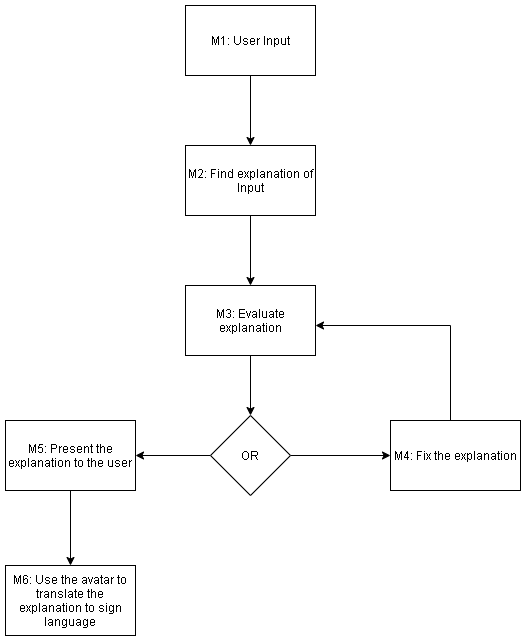
\includegraphics[scale=0.5]{ch4/assets/diagram1.png}
\caption[High-Level Approach]{High-Level Approach}
\label{fig:Diagram1}
\end{figure}

text

\begin{figure}[H]
\centering
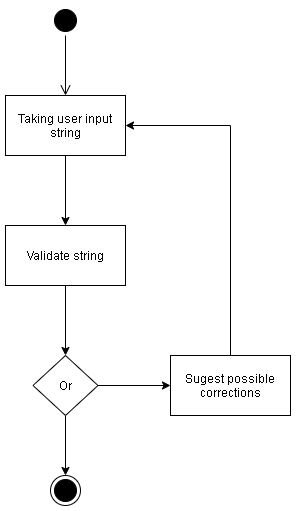
\includegraphics[scale=0.5]{ch4/assets/M1.png}
\caption[User Input Module]{M1: User Input}
\label{fig:M1}
\end{figure}

text

\begin{figure}[H]
\centering
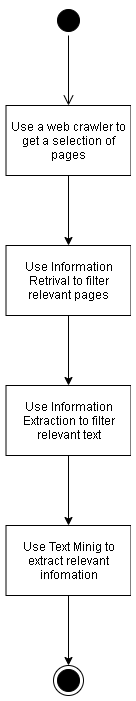
\includegraphics[scale=0.5]{ch4/assets/M2.png}
\caption[Find Explanation Module]{M2: Find Explanation}
\label{fig:M2}
\end{figure}

text

\begin{figure}[H]
\centering
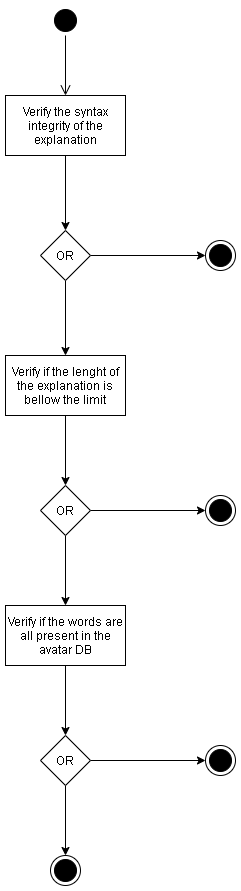
\includegraphics[scale=0.5]{ch4/assets/M3.png}
\caption[Evaluate Explanation Module]{M3: Evaluta Explanation}
\label{fig:M3}
\end{figure}

text

MISING M4

text

\begin{figure}[H]
\centering
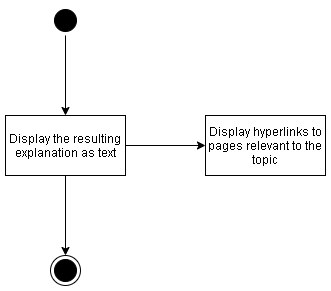
\includegraphics[scale=0.5]{ch4/assets/M5.png}
\caption[Present Explanation Module]{M5: Present Explanation}
\label{fig:M5}
\end{figure}

text

\begin{figure}[H]
\centering
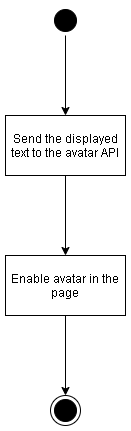
\includegraphics[scale=0.5]{ch4/assets/M6.png}
\caption[Avatar Module]{M6: Avatar}
\label{fig:M6}
\end{figure}